%----------------------------------------------------------------------------------------
%	SECTION 1.2
%----------------------------------------------------------------------------------------

\section{The Basis and Subbasis for a Topology.}

\begin{definition}
    If $X$ is a set, the \textbf{basis} for a topology on $X$ is a collection $\Bc$ of
    subsets of  $X$, called \textbf{basis elements}, such that:
        \begin{enumerate}
            \item[(1)] For every $x \in X$, there is a  $B \in \Bc$ such that $x \in B$.

            \item[(2)] For $B_1,B_2 \in \Bc$, if $x \in B_1 \cap B_2$, then there is a
                $B_3 \in \Bc$ such that $x \in B_3 \subseteq B_1 \cap B_2$
        \end{enumerate}
We define the topology $\Tc$ \textbf{generated} by $\Bc$ to be collection of open sets:
$\Tc=\{U \subseteq X: \text{for all } x \in U \text{, there exists a } B \in \Bc
\text{ such that } x \in B\}$.
\end{definition}

\begin{theorem}\label{1.2.1}
    Let $X$ be a set, and  $\Bc$ a basis of  $X$, then the collection of subsets
    of  $X$, $\Tc=\{U \subseteq X: \text{for all } x \in U \text{, there exists a
        } B \in \Bc \text{ such that } x \in B\}$ is a topology on $X$.
\end{theorem}
\begin{proof}
    Let $\Bc$ be a basis for a topology in  $X$, and consider  $\Tc$ as defined
    above. Cleary, $\emptyset \in X$ and so is  $X$.

    Now let  $\{U_{\alpha}\}$ be a collection of subsets of  $X$, and let
    $U=\bigcup{U_{\alpha}}$. Then if  $x \in U$ for some  $\alpha$, there is a
    $B_{\alpha}$ such that  $x \in B_{\alpha} \subseteq U_{\alpha}$, thus  $x \in
    B_{\alpha} \subseteq U$.

    Now let  $x \in  U_1 \cap U_2$, and choose $B_1,B_2 \in \Bc$ such that $x \in B_1 \subseteq U_1$
    and $x \in B_2 \subseteq U_2$. Then  by definition, there is a $B_3$ for which $x \in B_3 \subseteq B_1 \cap B_2$.
    Now suppose for arbitrary $n$, that  $U=\bigcap_{i=1}^{n}{U_i} \in \Tc$, for some finite
    collection  $\{U_i\}$ of subsets of  $X$. Then by let  $B_n, B_{n+1} \in \Bc$ such that
    $x \in B_n \subseteq U$ and  $x \in B_{n+1} \subseteq U_{n+1}$. Then by our hypothesis, there is a  $B$
for which  $x \in B \subseteq B_n \cap B_{n+1}$, thus  $U \cap U_{n+1}=\bigcap_{i=1}^{n+1}{U_i} \in \Tc$.
This make $\Tc$ a topology on  $X$.
\end{proof}

\begin{example}
    \begin{enumerate}
        \item[(1)] Let $\Bc$ be the set of all circular regions in the plane  $\R \times \R$, then
            $\Bc$ satisfies the conditions needed for a basis.

        \item[(2)] The collection  $\Bc'$ in  $\R \times \R$ of all rectangular region also
            forms a basis for a topology on  $\R \times \R$.

        \item[(3)] For any set  $X$, the set of all  $1$-point subsets of  $X$ forms a
            basis for a topology on  $X$.
    \end{enumerate}
\end{example}

\begin{figure}[h]
    \centering
    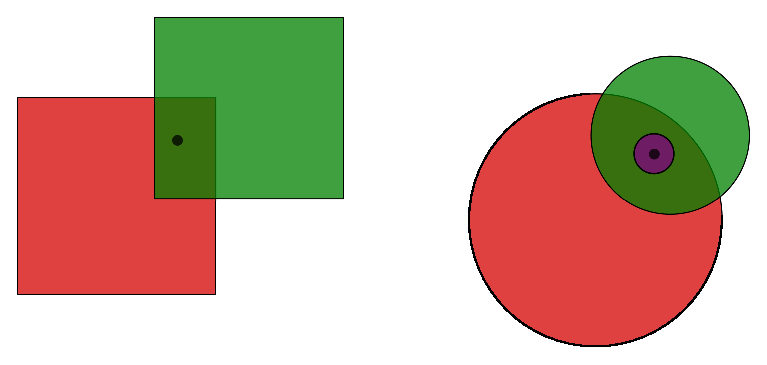
\includegraphics[scale = 0.5]{Figures/Chapter1/topology_basis.eps}
    \caption{The basis for $\Bc$ and  $\Bc'$ in  $\R \times \R$  (see example $(2)$).}
    \label{fig_1.2}
\end{figure}

\begin{lemma}\label{1.2.2}
    Let $X$ be a set, and  $\Bc$ be a basis for a topology  $\Tc$ on  $X$. Then
    $\Tc=\{\bigcup{B}: B \in \Bc\}$.
\end{lemma}
\begin{proof}
    Given a collection $\{B_i\}_{i=1}^{\infty}$ of basis elements in  $\Bc$, since they
    are all in  $\Tc$, their unions are also in $\Tc$. Conversely, given  $U \in \Tc$,
    then for every point $x \in U$, choose a  $B_x \in \B_x$ such that  $x \in B_x
    \subseteq U$, then  $U=\bigcup_{x \in U}{B_x}$.
\end{proof}

\begin{lemma}\label{1.2.3}
    Let $(X,\Tc)$ be a topological space, and let  $\Cc \subseteq \Tc$ be a collection
    of open sets of  $X$ such that for every  $x \in U$, there is a  $C \in \Cc$ such that
    $x \in  C \subseteq U$. Then  $\Cc$ is the basis for a $\Tc$ on  $X$.
\end{lemma}
\begin{proof}
    Take any $x \in X$, then there is a  $C \in \Cc$ such that 	$x \in C \subseteq U$,
    thus the first condition for a basis is satisfied. Now let  $x \in C_1 \cap C_2$ for
    $C_1, C_2 \in \Cc$, since $C_1 \cap C_2$ is open in $X$, there is a  $C_3 \in \Cc$ such that
    $x \in C_3 \subseteq C_1 \cap C_2$. Therefore $\Cc$ is a basis for a topology on  $X$.

    Now let $\Tc_\Cc$ be the the topology generated by  $\Cc$, now for  $U \in \Tc$, we have
    by the hypothesis, that  $U \in \Tc_\Cc$; and by lemma \ref{1.2.2},  $W \in \Tc_\Cc$ is the
    union of elements of  $\Cc$, which is a subcollection of  $\Tc$, thus  $W \in \Tc$. Therefore
     $\Tc_\Cc=\Tc$.
\end{proof}

\begin{lemma}\label{1.2.4}
    Let $\Bc$ and  $\Bc'$ be bases for topologies  $\Tc$ and  $\Tc'$ on  $X$. Then the
     $\Tc \subseteq \Tc'$ if and only if for all  $x \in X$, and all  $B \in \Bc$, there is a  $B' \in \Bc'$
     such that  $x \in B' \subseteq B$.
\end{lemma}
\begin{proof}
    Suppose first that $\Tc \subseteq \Tc'$, and let $x \in X$, and choose  $B \in \Bc$ such that
    $x \in B$, then  $B$ is open in  $\Tc$, thus it is open in  $\Tc'$, thus there is a
     $B' \in \Bc'$ such that  $x \in B' \subseteq B$. Conversely, suppose there is a  $B' \in \Bc'$
     for which  $x \in B' \subseteq B$ for all  $x \in X$,  $B \in \Bc$. Take  $x \in U \in \Tc$, since
      $\Bc$ generates  $\Tc$,  $x \in B \subseteq U$, since  $B' \subseteq B$, this implies that $U \in \Tc'$
      and $\Tc \subseteq \Tc'$.
\end{proof}

\begin{definition}
    If $\Bc$ is the collection of open intervals $(a,b)$ in  $\R$, we call the topology generated
    by  $\Bc$ the \textbf{standard topology} on $\R$, and we denote it simply by  $\R$.
\end{definition}

\begin{definition}
    If $\Bc$ is the collection of half open intervals  $[a,b)$ in  $\R$, we call the
    topology generated by  $\Bc$ the \textbf{lower limit topology} on $\R$, and we
    denote it simply by  $\R_l$. If $\Bc'$ is the collection of all half open intervals  $(a,b]$
    in  $\R$, then we call the topology generated by  $\Bc'$ the \textbf{upper limt topology}
    on $\R$, and denote it  $\R_L$.
\end{definition}

\begin{definition}
    If $\Bc$ is the collection of all open intervals of the form  $\com{(a,b)}{\ \frac{1}{\Z^+}}$,
    where $\frac{1}{\Z^+}=\{\frac{1}{n}: n \in \Z^+\}$, we call the topology generated by $\Bc$ the
    \textbf{$\frac{1}{\Z^+}$-topology} on $\R$, and we denote it  $\R_{\frac{1}{\Z^+}}$.
\end{definition}

\begin{lemma}\label{1.2.4}
    The topologies $\R_l$,  $\R_L$, and  $\R_{\frac{1}{\Z^+}}$ are all strictly finer than $\R$,
    but are not comparable with each other.
\end{lemma}
\begin{proof}
    Let $(a,b)$ be a basis element for  $\R$, and let  $x \in (a,b)$, the basis element $[x,b) \in \R_l$
    lies in $(a,b)$ and contains $x$, however, there can be no interval  $(a,b)$ in  $[x,b)$ as
     $x \leq a$, thus  $\R \subset \R_l$; a similar argument holds for  $\R_L$.

     Similarly, for  $(a,b) \in \R$, the basis element  $\com{(a,b)}{ \frac{1}{\Z^+}}$ of $\R_{\frac{1}{\Z^+}}$
     lies in $(a,b)$, however, choose the basis $B=\com{(-1,1)}{\frac{1}{\Z^+}}$, and
     choose $0 \in B$, since  $\Z^+$ is dense in  $\R$, there is no interval  $(a,b)$ containing  $0$
     and lying in  $B$, thus  $\R \subseteq \R_{\frac{1}{\Z^+}}$.

     Now choose $[0,1)$ in  $\R_l$, and choose  $ \frac{1}{k} \in [0,1)$ such that $k \in \Z^+$. Now
     $(0,1) \subseteq [0,1)]$, so we cannot say that $[0,1)$ is a basis for  $\R$, and moreover,
     $\com{[0,1)}{\frac{1}{\Z^+}}$ cannot be said to be a basis in $\R_{\frac{1}{\Z^+}}$, thus
     $\R_l$ and  $\R_{\frac{1}{\Z^+}}$ are incompararble, a similar argument holds for $\R_L$.

     Lastly, let  $(a,b)$ be in  $\R$ and choose  $x \in (a,b)$. Then $(a,x]$ and  $[x,b)$ are
     both in  $(a,b)$, however it is clear that  $(a,x]$ and  $[x,b)$ connot be contained in each other,
     thus $\R_l$ and  $\R_L$ are incomparable.
\end{proof}

\begin{definition}
    A \textbf{subbasis}, $\Sc$, for a topology on  $X$ is a collection of subsets of $X$ whose
    union equals $X$. We call the \textbf{topology generated by $\Sc$} to be the collection
    of all unions of finite intersections of elements of $\Sc$, that is:
        \begin{equation*}
            \Tc=\{\bigcup{\bigcap_{i=1}^{n}}{S_i}: S_i \in \Sc \text{ for } 1 \leq i \leq n\}
        \end{equation*}
\end{definition}

\begin{theorem}\label{1.2.5}
    Let $\Sc$ be a subbasis for a topology on  $X$. Then the collection $\Tc=\{\bigcup{\bigcap_{i=1}^{n}}{S_i}:
    S_i \in \Sc \text{ for } 1 \leq i \leq n\}$ is a topology on $X$.
\end{theorem}
\begin{proof}
    It is sufficient to show that the collection $\Bc$ of all finite intersections of elements
    of $\Sc$ is a basis for a topology on  $X$. By lemma \ref{1.2.1}, for $x \in X$, it belongs to
    an element  $S$ of  $\Sc$, and therefore, to an element of  $\Bc$. Now let  $B_1=\bigcap_{i=1}^m{S_i}$
    and $B_2=\bigcap_{j=1}^{n}{S'_j}$ be basis elements of $\Bc$. The intersection  $\B_1 \cap B_2$ is a
    finite intersection of elements of $\Sc$, and hence also belongs in  $\Bc$, and hence we can take
    another basis element  $B_3$ such that $x \in B_3 \subseteq B_1 \cap B_2$.
\end{proof}
